% Created by tikzDevice version 0.10.1 on 2016-09-07 16:42:15
% !TEX encoding = UTF-8 Unicode
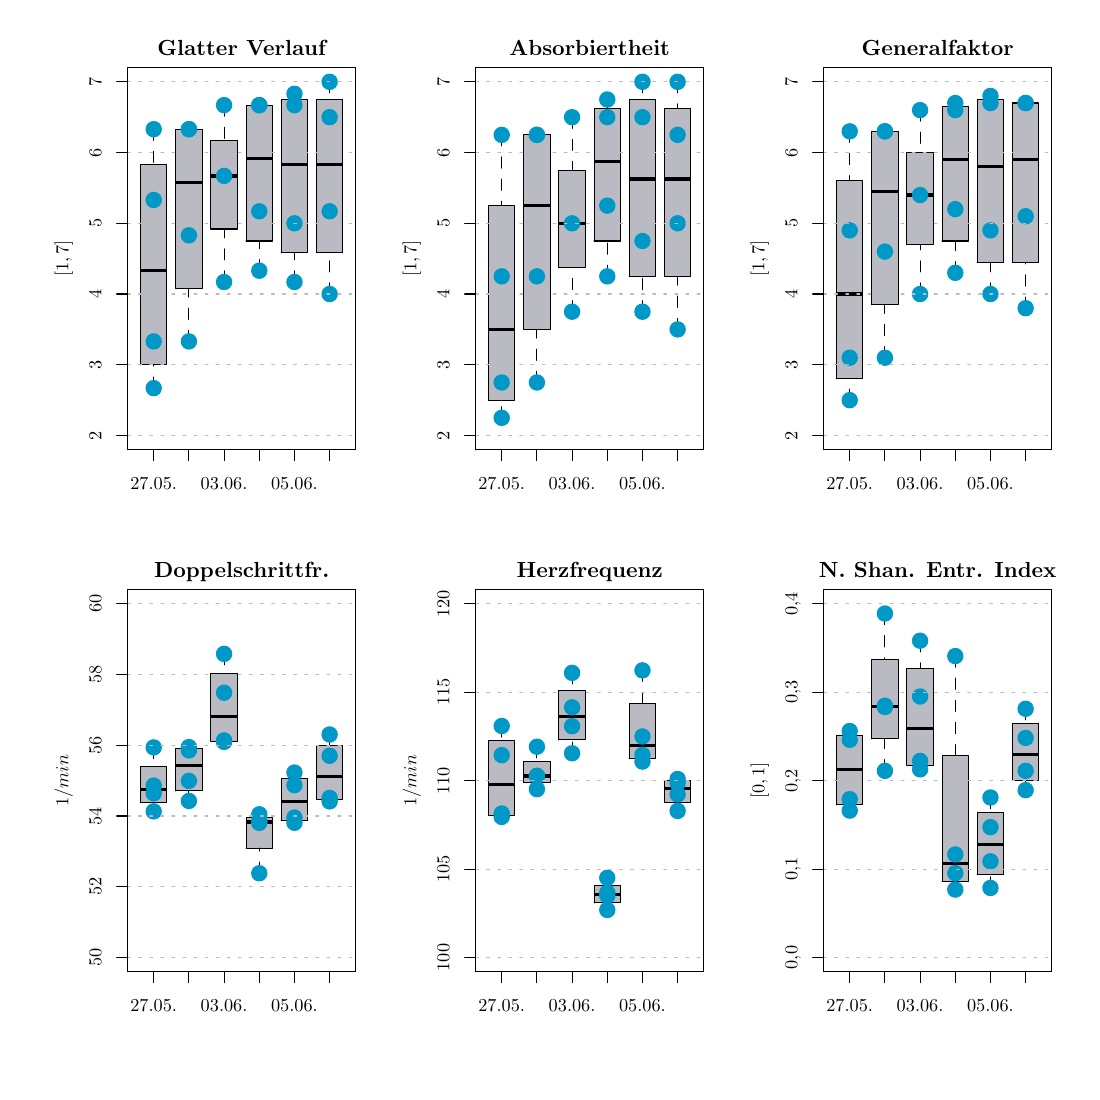
\begin{tikzpicture}[x=1pt,y=1pt]
\definecolor{fillColor}{RGB}{255,255,255}
\path[use as bounding box,fill=fillColor] (0,0) rectangle (377.25,377.25);
\begin{scope}
\path[clip] ( 36.13,224.76) rectangle (118.52,362.80);
\definecolor{fillColor}{RGB}{186,187,194}

\path[fill=fillColor] ( 40.78,255.43) --
	( 50.31,255.43) --
	( 50.31,327.78) --
	( 40.78,327.78) --
	cycle;
\definecolor{drawColor}{RGB}{0,0,0}

\path[draw=drawColor,line width= 1.2pt,line join=round] ( 40.78,289.43) -- ( 50.31,289.43);

\path[draw=drawColor,line width= 0.4pt,dash pattern=on 4pt off 4pt ,line join=round,line cap=round] ( 45.54,247.00) -- ( 45.54,255.43);

\path[draw=drawColor,line width= 0.4pt,dash pattern=on 4pt off 4pt ,line join=round,line cap=round] ( 45.54,340.56) -- ( 45.54,327.78);

\path[draw=drawColor,line width= 0.4pt,line join=round,line cap=round] ( 43.16,247.00) -- ( 47.93,247.00);

\path[draw=drawColor,line width= 0.4pt,line join=round,line cap=round] ( 43.16,340.56) -- ( 47.93,340.56);

\path[draw=drawColor,line width= 0.4pt,line join=round,line cap=round] ( 40.78,255.43) --
	( 50.31,255.43) --
	( 50.31,327.78) --
	( 40.78,327.78) --
	( 40.78,255.43);

\path[fill=fillColor] ( 53.49,283.04) --
	( 63.03,283.04) --
	( 63.03,340.56) --
	( 53.49,340.56) --
	cycle;

\path[draw=drawColor,line width= 1.2pt,line join=round] ( 53.49,321.38) -- ( 63.03,321.38);

\path[draw=drawColor,line width= 0.4pt,dash pattern=on 4pt off 4pt ,line join=round,line cap=round] ( 58.26,263.87) -- ( 58.26,283.04);

\path[draw=drawColor,line width= 0.4pt,dash pattern=on 4pt off 4pt ,line join=round,line cap=round] ( 58.26,340.56) -- ( 58.26,340.56);

\path[draw=drawColor,line width= 0.4pt,line join=round,line cap=round] ( 55.87,263.87) -- ( 60.64,263.87);

\path[draw=drawColor,line width= 0.4pt,line join=round,line cap=round] ( 55.87,340.56) -- ( 60.64,340.56);

\path[draw=drawColor,line width= 0.4pt,line join=round,line cap=round] ( 53.49,283.04) --
	( 63.03,283.04) --
	( 63.03,340.56) --
	( 53.49,340.56) --
	( 53.49,283.04);

\path[fill=fillColor] ( 66.20,304.51) --
	( 75.74,304.51) --
	( 75.74,336.47) --
	( 66.20,336.47) --
	cycle;

\path[draw=drawColor,line width= 1.2pt,line join=round] ( 66.20,323.69) -- ( 75.74,323.69);

\path[draw=drawColor,line width= 0.4pt,dash pattern=on 4pt off 4pt ,line join=round,line cap=round] ( 70.97,285.34) -- ( 70.97,304.51);

\path[draw=drawColor,line width= 0.4pt,dash pattern=on 4pt off 4pt ,line join=round,line cap=round] ( 70.97,349.25) -- ( 70.97,336.47);

\path[draw=drawColor,line width= 0.4pt,line join=round,line cap=round] ( 68.59,285.34) -- ( 73.36,285.34);

\path[draw=drawColor,line width= 0.4pt,line join=round,line cap=round] ( 68.59,349.25) -- ( 73.36,349.25);

\path[draw=drawColor,line width= 0.4pt,line join=round,line cap=round] ( 66.20,304.51) --
	( 75.74,304.51) --
	( 75.74,336.47) --
	( 66.20,336.47) --
	( 66.20,304.51);

\path[fill=fillColor] ( 78.92,300.17) --
	( 88.45,300.17) --
	( 88.45,349.25) --
	( 78.92,349.25) --
	cycle;

\path[draw=drawColor,line width= 1.2pt,line join=round] ( 78.92,330.08) -- ( 88.45,330.08);

\path[draw=drawColor,line width= 0.4pt,dash pattern=on 4pt off 4pt ,line join=round,line cap=round] ( 83.69,289.43) -- ( 83.69,300.17);

\path[draw=drawColor,line width= 0.4pt,dash pattern=on 4pt off 4pt ,line join=round,line cap=round] ( 83.69,349.25) -- ( 83.69,349.25);

\path[draw=drawColor,line width= 0.4pt,line join=round,line cap=round] ( 81.30,289.43) -- ( 86.07,289.43);

\path[draw=drawColor,line width= 0.4pt,line join=round,line cap=round] ( 81.30,349.25) -- ( 86.07,349.25);

\path[draw=drawColor,line width= 0.4pt,line join=round,line cap=round] ( 78.92,300.17) --
	( 88.45,300.17) --
	( 88.45,349.25) --
	( 78.92,349.25) --
	( 78.92,300.17);

\path[fill=fillColor] ( 91.63,295.95) --
	(101.17,295.95) --
	(101.17,351.29) --
	( 91.63,351.29) --
	cycle;

\path[draw=drawColor,line width= 1.2pt,line join=round] ( 91.63,327.90) -- (101.17,327.90);

\path[draw=drawColor,line width= 0.4pt,dash pattern=on 4pt off 4pt ,line join=round,line cap=round] ( 96.40,285.34) -- ( 96.40,295.95);

\path[draw=drawColor,line width= 0.4pt,dash pattern=on 4pt off 4pt ,line join=round,line cap=round] ( 96.40,353.34) -- ( 96.40,351.29);

\path[draw=drawColor,line width= 0.4pt,line join=round,line cap=round] ( 94.02,285.34) -- ( 98.78,285.34);

\path[draw=drawColor,line width= 0.4pt,line join=round,line cap=round] ( 94.02,353.34) -- ( 98.78,353.34);

\path[draw=drawColor,line width= 0.4pt,line join=round,line cap=round] ( 91.63,295.95) --
	(101.17,295.95) --
	(101.17,351.29) --
	( 91.63,351.29) --
	( 91.63,295.95);

\path[fill=fillColor] (104.35,295.95) --
	(113.88,295.95) --
	(113.88,351.29) --
	(104.35,351.29) --
	cycle;

\path[draw=drawColor,line width= 1.2pt,line join=round] (104.35,327.90) -- (113.88,327.90);

\path[draw=drawColor,line width= 0.4pt,dash pattern=on 4pt off 4pt ,line join=round,line cap=round] (109.11,281.00) -- (109.11,295.95);

\path[draw=drawColor,line width= 0.4pt,dash pattern=on 4pt off 4pt ,line join=round,line cap=round] (109.11,357.68) -- (109.11,351.29);

\path[draw=drawColor,line width= 0.4pt,line join=round,line cap=round] (106.73,281.00) -- (111.50,281.00);

\path[draw=drawColor,line width= 0.4pt,line join=round,line cap=round] (106.73,357.68) -- (111.50,357.68);

\path[draw=drawColor,line width= 0.4pt,line join=round,line cap=round] (104.35,295.95) --
	(113.88,295.95) --
	(113.88,351.29) --
	(104.35,351.29) --
	(104.35,295.95);
\end{scope}
\begin{scope}
\path[clip] (  0.00,  0.00) rectangle (377.25,377.25);
\definecolor{drawColor}{RGB}{0,0,0}

\path[draw=drawColor,line width= 0.4pt,line join=round,line cap=round] ( 45.54,224.76) -- (109.11,224.76);

\path[draw=drawColor,line width= 0.4pt,line join=round,line cap=round] ( 45.54,224.76) -- ( 45.54,220.80);

\path[draw=drawColor,line width= 0.4pt,line join=round,line cap=round] ( 58.26,224.76) -- ( 58.26,220.80);

\path[draw=drawColor,line width= 0.4pt,line join=round,line cap=round] ( 70.97,224.76) -- ( 70.97,220.80);

\path[draw=drawColor,line width= 0.4pt,line join=round,line cap=round] ( 83.69,224.76) -- ( 83.69,220.80);

\path[draw=drawColor,line width= 0.4pt,line join=round,line cap=round] ( 96.40,224.76) -- ( 96.40,220.80);

\path[draw=drawColor,line width= 0.4pt,line join=round,line cap=round] (109.11,224.76) -- (109.11,220.80);

\node[text=drawColor,anchor=base,inner sep=0pt, outer sep=0pt, scale=  0.66] at ( 45.54,210.50) {27.05.};

\node[text=drawColor,anchor=base,inner sep=0pt, outer sep=0pt, scale=  0.66] at ( 70.97,210.50) {03.06.};

\node[text=drawColor,anchor=base,inner sep=0pt, outer sep=0pt, scale=  0.66] at ( 96.40,210.50) {05.06.};

\path[draw=drawColor,line width= 0.4pt,line join=round,line cap=round] ( 36.13,229.87) -- ( 36.13,357.68);

\path[draw=drawColor,line width= 0.4pt,line join=round,line cap=round] ( 36.13,229.87) -- ( 32.17,229.87);

\path[draw=drawColor,line width= 0.4pt,line join=round,line cap=round] ( 36.13,255.43) -- ( 32.17,255.43);

\path[draw=drawColor,line width= 0.4pt,line join=round,line cap=round] ( 36.13,281.00) -- ( 32.17,281.00);

\path[draw=drawColor,line width= 0.4pt,line join=round,line cap=round] ( 36.13,306.56) -- ( 32.17,306.56);

\path[draw=drawColor,line width= 0.4pt,line join=round,line cap=round] ( 36.13,332.12) -- ( 32.17,332.12);

\path[draw=drawColor,line width= 0.4pt,line join=round,line cap=round] ( 36.13,357.68) -- ( 32.17,357.68);

\node[text=drawColor,rotate= 90.00,anchor=base,inner sep=0pt, outer sep=0pt, scale=  0.66] at ( 26.63,229.87) {2};

\node[text=drawColor,rotate= 90.00,anchor=base,inner sep=0pt, outer sep=0pt, scale=  0.66] at ( 26.63,255.43) {3};

\node[text=drawColor,rotate= 90.00,anchor=base,inner sep=0pt, outer sep=0pt, scale=  0.66] at ( 26.63,281.00) {4};

\node[text=drawColor,rotate= 90.00,anchor=base,inner sep=0pt, outer sep=0pt, scale=  0.66] at ( 26.63,306.56) {5};

\node[text=drawColor,rotate= 90.00,anchor=base,inner sep=0pt, outer sep=0pt, scale=  0.66] at ( 26.63,332.12) {6};

\node[text=drawColor,rotate= 90.00,anchor=base,inner sep=0pt, outer sep=0pt, scale=  0.66] at ( 26.63,357.68) {7};
\end{scope}
\begin{scope}
\path[clip] (  0.00,188.62) rectangle (125.75,377.25);
\definecolor{drawColor}{RGB}{0,0,0}

\node[text=drawColor,anchor=base,inner sep=0pt, outer sep=0pt, scale=  0.79] at ( 77.33,367.29) {\bfseries Glatter Verlauf};

\node[text=drawColor,rotate= 90.00,anchor=base,inner sep=0pt, outer sep=0pt, scale=  0.66] at ( 14.75,293.78) {$[1, 7]$};
\end{scope}
\begin{scope}
\path[clip] (  0.00,  0.00) rectangle (377.25,377.25);
\definecolor{drawColor}{RGB}{0,0,0}

\path[draw=drawColor,line width= 0.4pt,line join=round,line cap=round] ( 36.13,224.76) --
	(118.52,224.76) --
	(118.52,362.80) --
	( 36.13,362.80) --
	( 36.13,224.76);
\end{scope}
\begin{scope}
\path[clip] ( 36.13,224.76) rectangle (118.52,362.80);
\definecolor{fillColor}{RGB}{0,152,199}

\path[fill=fillColor] ( 45.54,247.00) circle (  2.97);

\path[fill=fillColor] ( 45.54,263.87) circle (  2.97);

\path[fill=fillColor] ( 45.54,314.99) circle (  2.97);

\path[fill=fillColor] ( 45.54,340.56) circle (  2.97);

\path[fill=fillColor] ( 58.26,263.87) circle (  2.97);

\path[fill=fillColor] ( 58.26,302.21) circle (  2.97);

\path[fill=fillColor] ( 58.26,340.56) circle (  2.97);

\path[fill=fillColor] ( 58.26,340.56) circle (  2.97);

\path[fill=fillColor] ( 70.97,285.34) circle (  2.97);

\path[fill=fillColor] ( 70.97,323.69) circle (  2.97);

\path[fill=fillColor] ( 70.97,349.25) circle (  2.97);

\path[fill=fillColor] ( 83.69,289.43) circle (  2.97);

\path[fill=fillColor] ( 83.69,310.90) circle (  2.97);

\path[fill=fillColor] ( 83.69,349.25) circle (  2.97);

\path[fill=fillColor] ( 83.69,349.25) circle (  2.97);

\path[fill=fillColor] ( 96.40,285.34) circle (  2.97);

\path[fill=fillColor] ( 96.40,306.56) circle (  2.97);

\path[fill=fillColor] ( 96.40,353.34) circle (  2.97);

\path[fill=fillColor] ( 96.40,349.25) circle (  2.97);

\path[fill=fillColor] (109.11,281.00) circle (  2.97);

\path[fill=fillColor] (109.11,310.90) circle (  2.97);

\path[fill=fillColor] (109.11,344.90) circle (  2.97);

\path[fill=fillColor] (109.11,357.68) circle (  2.97);
\definecolor{drawColor}{RGB}{186,187,194}

\path[draw=drawColor,line width= 0.4pt,dash pattern=on 1pt off 3pt ,line join=round,line cap=round] ( 36.13,229.87) -- (118.52,229.87);

\path[draw=drawColor,line width= 0.4pt,dash pattern=on 1pt off 3pt ,line join=round,line cap=round] ( 36.13,255.43) -- (118.52,255.43);

\path[draw=drawColor,line width= 0.4pt,dash pattern=on 1pt off 3pt ,line join=round,line cap=round] ( 36.13,281.00) -- (118.52,281.00);

\path[draw=drawColor,line width= 0.4pt,dash pattern=on 1pt off 3pt ,line join=round,line cap=round] ( 36.13,306.56) -- (118.52,306.56);

\path[draw=drawColor,line width= 0.4pt,dash pattern=on 1pt off 3pt ,line join=round,line cap=round] ( 36.13,332.12) -- (118.52,332.12);

\path[draw=drawColor,line width= 0.4pt,dash pattern=on 1pt off 3pt ,line join=round,line cap=round] ( 36.13,357.68) -- (118.52,357.68);
\end{scope}
\begin{scope}
\path[clip] (  0.00,  0.00) rectangle (377.25,377.25);
\definecolor{drawColor}{RGB}{0,0,0}

\path[draw=drawColor,line width= 0.4pt,line join=round,line cap=round] ( 36.13,224.76) --
	(118.52,224.76) --
	(118.52,362.80) --
	( 36.13,362.80) --
	( 36.13,224.76);
\end{scope}
\begin{scope}
\path[clip] (161.88,224.76) rectangle (244.27,362.80);
\definecolor{fillColor}{RGB}{186,187,194}

\path[fill=fillColor] (166.53,242.65) --
	(176.06,242.65) --
	(176.06,312.95) --
	(166.53,312.95) --
	cycle;
\definecolor{drawColor}{RGB}{0,0,0}

\path[draw=drawColor,line width= 1.2pt,line join=round] (166.53,268.22) -- (176.06,268.22);

\path[draw=drawColor,line width= 0.4pt,dash pattern=on 4pt off 4pt ,line join=round,line cap=round] (171.29,236.26) -- (171.29,242.65);

\path[draw=drawColor,line width= 0.4pt,dash pattern=on 4pt off 4pt ,line join=round,line cap=round] (171.29,338.51) -- (171.29,312.95);

\path[draw=drawColor,line width= 0.4pt,line join=round,line cap=round] (168.91,236.26) -- (173.68,236.26);

\path[draw=drawColor,line width= 0.4pt,line join=round,line cap=round] (168.91,338.51) -- (173.68,338.51);

\path[draw=drawColor,line width= 0.4pt,line join=round,line cap=round] (166.53,242.65) --
	(176.06,242.65) --
	(176.06,312.95) --
	(166.53,312.95) --
	(166.53,242.65);

\path[fill=fillColor] (179.24,268.22) --
	(188.78,268.22) --
	(188.78,338.51) --
	(179.24,338.51) --
	cycle;

\path[draw=drawColor,line width= 1.2pt,line join=round] (179.24,312.95) -- (188.78,312.95);

\path[draw=drawColor,line width= 0.4pt,dash pattern=on 4pt off 4pt ,line join=round,line cap=round] (184.01,249.04) -- (184.01,268.22);

\path[draw=drawColor,line width= 0.4pt,dash pattern=on 4pt off 4pt ,line join=round,line cap=round] (184.01,338.51) -- (184.01,338.51);

\path[draw=drawColor,line width= 0.4pt,line join=round,line cap=round] (181.62,249.04) -- (186.39,249.04);

\path[draw=drawColor,line width= 0.4pt,line join=round,line cap=round] (181.62,338.51) -- (186.39,338.51);

\path[draw=drawColor,line width= 0.4pt,line join=round,line cap=round] (179.24,268.22) --
	(188.78,268.22) --
	(188.78,338.51) --
	(179.24,338.51) --
	(179.24,268.22);

\path[fill=fillColor] (191.95,290.58) --
	(201.49,290.58) --
	(201.49,325.73) --
	(191.95,325.73) --
	cycle;

\path[draw=drawColor,line width= 1.2pt,line join=round] (191.95,306.56) -- (201.49,306.56);

\path[draw=drawColor,line width= 0.4pt,dash pattern=on 4pt off 4pt ,line join=round,line cap=round] (196.72,274.61) -- (196.72,290.58);

\path[draw=drawColor,line width= 0.4pt,dash pattern=on 4pt off 4pt ,line join=round,line cap=round] (196.72,344.90) -- (196.72,325.73);

\path[draw=drawColor,line width= 0.4pt,line join=round,line cap=round] (194.34,274.61) -- (199.11,274.61);

\path[draw=drawColor,line width= 0.4pt,line join=round,line cap=round] (194.34,344.90) -- (199.11,344.90);

\path[draw=drawColor,line width= 0.4pt,line join=round,line cap=round] (191.95,290.58) --
	(201.49,290.58) --
	(201.49,325.73) --
	(191.95,325.73) --
	(191.95,290.58);

\path[fill=fillColor] (204.67,300.17) --
	(214.20,300.17) --
	(214.20,348.10) --
	(204.67,348.10) --
	cycle;

\path[draw=drawColor,line width= 1.2pt,line join=round] (204.67,328.93) -- (214.20,328.93);

\path[draw=drawColor,line width= 0.4pt,dash pattern=on 4pt off 4pt ,line join=round,line cap=round] (209.44,287.39) -- (209.44,300.17);

\path[draw=drawColor,line width= 0.4pt,dash pattern=on 4pt off 4pt ,line join=round,line cap=round] (209.44,351.29) -- (209.44,348.10);

\path[draw=drawColor,line width= 0.4pt,line join=round,line cap=round] (207.05,287.39) -- (211.82,287.39);

\path[draw=drawColor,line width= 0.4pt,line join=round,line cap=round] (207.05,351.29) -- (211.82,351.29);

\path[draw=drawColor,line width= 0.4pt,line join=round,line cap=round] (204.67,300.17) --
	(214.20,300.17) --
	(214.20,348.10) --
	(204.67,348.10) --
	(204.67,300.17);

\path[fill=fillColor] (217.38,287.39) --
	(226.92,287.39) --
	(226.92,351.29) --
	(217.38,351.29) --
	cycle;

\path[draw=drawColor,line width= 1.2pt,line join=round] (217.38,322.53) -- (226.92,322.53);

\path[draw=drawColor,line width= 0.4pt,dash pattern=on 4pt off 4pt ,line join=round,line cap=round] (222.15,274.61) -- (222.15,287.39);

\path[draw=drawColor,line width= 0.4pt,dash pattern=on 4pt off 4pt ,line join=round,line cap=round] (222.15,357.68) -- (222.15,351.29);

\path[draw=drawColor,line width= 0.4pt,line join=round,line cap=round] (219.77,274.61) -- (224.53,274.61);

\path[draw=drawColor,line width= 0.4pt,line join=round,line cap=round] (219.77,357.68) -- (224.53,357.68);

\path[draw=drawColor,line width= 0.4pt,line join=round,line cap=round] (217.38,287.39) --
	(226.92,287.39) --
	(226.92,351.29) --
	(217.38,351.29) --
	(217.38,287.39);

\path[fill=fillColor] (230.10,287.39) --
	(239.63,287.39) --
	(239.63,348.10) --
	(230.10,348.10) --
	cycle;

\path[draw=drawColor,line width= 1.2pt,line join=round] (230.10,322.53) -- (239.63,322.53);

\path[draw=drawColor,line width= 0.4pt,dash pattern=on 4pt off 4pt ,line join=round,line cap=round] (234.86,268.22) -- (234.86,287.39);

\path[draw=drawColor,line width= 0.4pt,dash pattern=on 4pt off 4pt ,line join=round,line cap=round] (234.86,357.68) -- (234.86,348.10);

\path[draw=drawColor,line width= 0.4pt,line join=round,line cap=round] (232.48,268.22) -- (237.25,268.22);

\path[draw=drawColor,line width= 0.4pt,line join=round,line cap=round] (232.48,357.68) -- (237.25,357.68);

\path[draw=drawColor,line width= 0.4pt,line join=round,line cap=round] (230.10,287.39) --
	(239.63,287.39) --
	(239.63,348.10) --
	(230.10,348.10) --
	(230.10,287.39);
\end{scope}
\begin{scope}
\path[clip] (  0.00,  0.00) rectangle (377.25,377.25);
\definecolor{drawColor}{RGB}{0,0,0}

\path[draw=drawColor,line width= 0.4pt,line join=round,line cap=round] (171.29,224.76) -- (234.86,224.76);

\path[draw=drawColor,line width= 0.4pt,line join=round,line cap=round] (171.29,224.76) -- (171.29,220.80);

\path[draw=drawColor,line width= 0.4pt,line join=round,line cap=round] (184.01,224.76) -- (184.01,220.80);

\path[draw=drawColor,line width= 0.4pt,line join=round,line cap=round] (196.72,224.76) -- (196.72,220.80);

\path[draw=drawColor,line width= 0.4pt,line join=round,line cap=round] (209.44,224.76) -- (209.44,220.80);

\path[draw=drawColor,line width= 0.4pt,line join=round,line cap=round] (222.15,224.76) -- (222.15,220.80);

\path[draw=drawColor,line width= 0.4pt,line join=round,line cap=round] (234.86,224.76) -- (234.86,220.80);

\node[text=drawColor,anchor=base,inner sep=0pt, outer sep=0pt, scale=  0.66] at (171.29,210.50) {27.05.};

\node[text=drawColor,anchor=base,inner sep=0pt, outer sep=0pt, scale=  0.66] at (196.72,210.50) {03.06.};

\node[text=drawColor,anchor=base,inner sep=0pt, outer sep=0pt, scale=  0.66] at (222.15,210.50) {05.06.};

\path[draw=drawColor,line width= 0.4pt,line join=round,line cap=round] (161.88,229.87) -- (161.88,357.68);

\path[draw=drawColor,line width= 0.4pt,line join=round,line cap=round] (161.88,229.87) -- (157.92,229.87);

\path[draw=drawColor,line width= 0.4pt,line join=round,line cap=round] (161.88,255.43) -- (157.92,255.43);

\path[draw=drawColor,line width= 0.4pt,line join=round,line cap=round] (161.88,281.00) -- (157.92,281.00);

\path[draw=drawColor,line width= 0.4pt,line join=round,line cap=round] (161.88,306.56) -- (157.92,306.56);

\path[draw=drawColor,line width= 0.4pt,line join=round,line cap=round] (161.88,332.12) -- (157.92,332.12);

\path[draw=drawColor,line width= 0.4pt,line join=round,line cap=round] (161.88,357.68) -- (157.92,357.68);

\node[text=drawColor,rotate= 90.00,anchor=base,inner sep=0pt, outer sep=0pt, scale=  0.66] at (152.38,229.87) {2};

\node[text=drawColor,rotate= 90.00,anchor=base,inner sep=0pt, outer sep=0pt, scale=  0.66] at (152.38,255.43) {3};

\node[text=drawColor,rotate= 90.00,anchor=base,inner sep=0pt, outer sep=0pt, scale=  0.66] at (152.38,281.00) {4};

\node[text=drawColor,rotate= 90.00,anchor=base,inner sep=0pt, outer sep=0pt, scale=  0.66] at (152.38,306.56) {5};

\node[text=drawColor,rotate= 90.00,anchor=base,inner sep=0pt, outer sep=0pt, scale=  0.66] at (152.38,332.12) {6};

\node[text=drawColor,rotate= 90.00,anchor=base,inner sep=0pt, outer sep=0pt, scale=  0.66] at (152.38,357.68) {7};
\end{scope}
\begin{scope}
\path[clip] (125.75,188.62) rectangle (251.50,377.25);
\definecolor{drawColor}{RGB}{0,0,0}

\node[text=drawColor,anchor=base,inner sep=0pt, outer sep=0pt, scale=  0.79] at (203.08,367.29) {\bfseries Absorbiertheit};

\node[text=drawColor,rotate= 90.00,anchor=base,inner sep=0pt, outer sep=0pt, scale=  0.66] at (140.50,293.78) {$[1, 7]$};
\end{scope}
\begin{scope}
\path[clip] (  0.00,  0.00) rectangle (377.25,377.25);
\definecolor{drawColor}{RGB}{0,0,0}

\path[draw=drawColor,line width= 0.4pt,line join=round,line cap=round] (161.88,224.76) --
	(244.27,224.76) --
	(244.27,362.80) --
	(161.88,362.80) --
	(161.88,224.76);
\end{scope}
\begin{scope}
\path[clip] (161.88,224.76) rectangle (244.27,362.80);
\definecolor{fillColor}{RGB}{0,152,199}

\path[fill=fillColor] (171.29,236.26) circle (  2.97);

\path[fill=fillColor] (171.29,249.04) circle (  2.97);

\path[fill=fillColor] (171.29,287.39) circle (  2.97);

\path[fill=fillColor] (171.29,338.51) circle (  2.97);

\path[fill=fillColor] (184.01,249.04) circle (  2.97);

\path[fill=fillColor] (184.01,287.39) circle (  2.97);

\path[fill=fillColor] (184.01,338.51) circle (  2.97);

\path[fill=fillColor] (184.01,338.51) circle (  2.97);

\path[fill=fillColor] (196.72,274.61) circle (  2.97);

\path[fill=fillColor] (196.72,306.56) circle (  2.97);

\path[fill=fillColor] (196.72,344.90) circle (  2.97);

\path[fill=fillColor] (209.44,287.39) circle (  2.97);

\path[fill=fillColor] (209.44,312.95) circle (  2.97);

\path[fill=fillColor] (209.44,344.90) circle (  2.97);

\path[fill=fillColor] (209.44,351.29) circle (  2.97);

\path[fill=fillColor] (222.15,274.61) circle (  2.97);

\path[fill=fillColor] (222.15,300.17) circle (  2.97);

\path[fill=fillColor] (222.15,344.90) circle (  2.97);

\path[fill=fillColor] (222.15,357.68) circle (  2.97);

\path[fill=fillColor] (234.86,268.22) circle (  2.97);

\path[fill=fillColor] (234.86,306.56) circle (  2.97);

\path[fill=fillColor] (234.86,357.68) circle (  2.97);

\path[fill=fillColor] (234.86,338.51) circle (  2.97);
\definecolor{drawColor}{RGB}{186,187,194}

\path[draw=drawColor,line width= 0.4pt,dash pattern=on 1pt off 3pt ,line join=round,line cap=round] (161.88,229.87) -- (244.27,229.87);

\path[draw=drawColor,line width= 0.4pt,dash pattern=on 1pt off 3pt ,line join=round,line cap=round] (161.88,255.43) -- (244.27,255.43);

\path[draw=drawColor,line width= 0.4pt,dash pattern=on 1pt off 3pt ,line join=round,line cap=round] (161.88,281.00) -- (244.27,281.00);

\path[draw=drawColor,line width= 0.4pt,dash pattern=on 1pt off 3pt ,line join=round,line cap=round] (161.88,306.56) -- (244.27,306.56);

\path[draw=drawColor,line width= 0.4pt,dash pattern=on 1pt off 3pt ,line join=round,line cap=round] (161.88,332.12) -- (244.27,332.12);

\path[draw=drawColor,line width= 0.4pt,dash pattern=on 1pt off 3pt ,line join=round,line cap=round] (161.88,357.68) -- (244.27,357.68);
\end{scope}
\begin{scope}
\path[clip] (  0.00,  0.00) rectangle (377.25,377.25);
\definecolor{drawColor}{RGB}{0,0,0}

\path[draw=drawColor,line width= 0.4pt,line join=round,line cap=round] (161.88,224.76) --
	(244.27,224.76) --
	(244.27,362.80) --
	(161.88,362.80) --
	(161.88,224.76);
\end{scope}
\begin{scope}
\path[clip] (287.63,224.76) rectangle (370.02,362.80);
\definecolor{fillColor}{RGB}{186,187,194}

\path[fill=fillColor] (292.28,250.32) --
	(301.81,250.32) --
	(301.81,321.90) --
	(292.28,321.90) --
	cycle;
\definecolor{drawColor}{RGB}{0,0,0}

\path[draw=drawColor,line width= 1.2pt,line join=round] (292.28,281.00) -- (301.81,281.00);

\path[draw=drawColor,line width= 0.4pt,dash pattern=on 4pt off 4pt ,line join=round,line cap=round] (297.04,242.65) -- (297.04,250.32);

\path[draw=drawColor,line width= 0.4pt,dash pattern=on 4pt off 4pt ,line join=round,line cap=round] (297.04,339.79) -- (297.04,321.90);

\path[draw=drawColor,line width= 0.4pt,line join=round,line cap=round] (294.66,242.65) -- (299.43,242.65);

\path[draw=drawColor,line width= 0.4pt,line join=round,line cap=round] (294.66,339.79) -- (299.43,339.79);

\path[draw=drawColor,line width= 0.4pt,line join=round,line cap=round] (292.28,250.32) --
	(301.81,250.32) --
	(301.81,321.90) --
	(292.28,321.90) --
	(292.28,250.32);

\path[fill=fillColor] (304.99,277.16) --
	(314.53,277.16) --
	(314.53,339.79) --
	(304.99,339.79) --
	cycle;

\path[draw=drawColor,line width= 1.2pt,line join=round] (304.99,318.06) -- (314.53,318.06);

\path[draw=drawColor,line width= 0.4pt,dash pattern=on 4pt off 4pt ,line join=round,line cap=round] (309.76,257.99) -- (309.76,277.16);

\path[draw=drawColor,line width= 0.4pt,dash pattern=on 4pt off 4pt ,line join=round,line cap=round] (309.76,339.79) -- (309.76,339.79);

\path[draw=drawColor,line width= 0.4pt,line join=round,line cap=round] (307.37,257.99) -- (312.14,257.99);

\path[draw=drawColor,line width= 0.4pt,line join=round,line cap=round] (307.37,339.79) -- (312.14,339.79);

\path[draw=drawColor,line width= 0.4pt,line join=round,line cap=round] (304.99,277.16) --
	(314.53,277.16) --
	(314.53,339.79) --
	(304.99,339.79) --
	(304.99,277.16);

\path[fill=fillColor] (317.70,298.89) --
	(327.24,298.89) --
	(327.24,332.12) --
	(317.70,332.12) --
	cycle;

\path[draw=drawColor,line width= 1.2pt,line join=round] (317.70,316.78) -- (327.24,316.78);

\path[draw=drawColor,line width= 0.4pt,dash pattern=on 4pt off 4pt ,line join=round,line cap=round] (322.47,281.00) -- (322.47,298.89);

\path[draw=drawColor,line width= 0.4pt,dash pattern=on 4pt off 4pt ,line join=round,line cap=round] (322.47,347.46) -- (322.47,332.12);

\path[draw=drawColor,line width= 0.4pt,line join=round,line cap=round] (320.09,281.00) -- (324.86,281.00);

\path[draw=drawColor,line width= 0.4pt,line join=round,line cap=round] (320.09,347.46) -- (324.86,347.46);

\path[draw=drawColor,line width= 0.4pt,line join=round,line cap=round] (317.70,298.89) --
	(327.24,298.89) --
	(327.24,332.12) --
	(317.70,332.12) --
	(317.70,298.89);

\path[fill=fillColor] (330.42,300.17) --
	(339.95,300.17) --
	(339.95,348.74) --
	(330.42,348.74) --
	cycle;

\path[draw=drawColor,line width= 1.2pt,line join=round] (330.42,329.56) -- (339.95,329.56);

\path[draw=drawColor,line width= 0.4pt,dash pattern=on 4pt off 4pt ,line join=round,line cap=round] (335.19,288.67) -- (335.19,300.17);

\path[draw=drawColor,line width= 0.4pt,dash pattern=on 4pt off 4pt ,line join=round,line cap=round] (335.19,350.01) -- (335.19,348.74);

\path[draw=drawColor,line width= 0.4pt,line join=round,line cap=round] (332.80,288.67) -- (337.57,288.67);

\path[draw=drawColor,line width= 0.4pt,line join=round,line cap=round] (332.80,350.01) -- (337.57,350.01);

\path[draw=drawColor,line width= 0.4pt,line join=round,line cap=round] (330.42,300.17) --
	(339.95,300.17) --
	(339.95,348.74) --
	(330.42,348.74) --
	(330.42,300.17);

\path[fill=fillColor] (343.13,292.50) --
	(352.67,292.50) --
	(352.67,351.29) --
	(343.13,351.29) --
	cycle;

\path[draw=drawColor,line width= 1.2pt,line join=round] (343.13,327.01) -- (352.67,327.01);

\path[draw=drawColor,line width= 0.4pt,dash pattern=on 4pt off 4pt ,line join=round,line cap=round] (347.90,281.00) -- (347.90,292.50);

\path[draw=drawColor,line width= 0.4pt,dash pattern=on 4pt off 4pt ,line join=round,line cap=round] (347.90,352.57) -- (347.90,351.29);

\path[draw=drawColor,line width= 0.4pt,line join=round,line cap=round] (345.52,281.00) -- (350.28,281.00);

\path[draw=drawColor,line width= 0.4pt,line join=round,line cap=round] (345.52,352.57) -- (350.28,352.57);

\path[draw=drawColor,line width= 0.4pt,line join=round,line cap=round] (343.13,292.50) --
	(352.67,292.50) --
	(352.67,351.29) --
	(343.13,351.29) --
	(343.13,292.50);

\path[fill=fillColor] (355.85,292.50) --
	(365.38,292.50) --
	(365.38,350.01) --
	(355.85,350.01) --
	cycle;

\path[draw=drawColor,line width= 1.2pt,line join=round] (355.85,329.56) -- (365.38,329.56);

\path[draw=drawColor,line width= 0.4pt,dash pattern=on 4pt off 4pt ,line join=round,line cap=round] (360.61,275.88) -- (360.61,292.50);

\path[draw=drawColor,line width= 0.4pt,dash pattern=on 4pt off 4pt ,line join=round,line cap=round] (360.61,350.01) -- (360.61,350.01);

\path[draw=drawColor,line width= 0.4pt,line join=round,line cap=round] (358.23,275.88) -- (363.00,275.88);

\path[draw=drawColor,line width= 0.4pt,line join=round,line cap=round] (358.23,350.01) -- (363.00,350.01);

\path[draw=drawColor,line width= 0.4pt,line join=round,line cap=round] (355.85,292.50) --
	(365.38,292.50) --
	(365.38,350.01) --
	(355.85,350.01) --
	(355.85,292.50);
\end{scope}
\begin{scope}
\path[clip] (  0.00,  0.00) rectangle (377.25,377.25);
\definecolor{drawColor}{RGB}{0,0,0}

\path[draw=drawColor,line width= 0.4pt,line join=round,line cap=round] (297.04,224.76) -- (360.61,224.76);

\path[draw=drawColor,line width= 0.4pt,line join=round,line cap=round] (297.04,224.76) -- (297.04,220.80);

\path[draw=drawColor,line width= 0.4pt,line join=round,line cap=round] (309.76,224.76) -- (309.76,220.80);

\path[draw=drawColor,line width= 0.4pt,line join=round,line cap=round] (322.47,224.76) -- (322.47,220.80);

\path[draw=drawColor,line width= 0.4pt,line join=round,line cap=round] (335.19,224.76) -- (335.19,220.80);

\path[draw=drawColor,line width= 0.4pt,line join=round,line cap=round] (347.90,224.76) -- (347.90,220.80);

\path[draw=drawColor,line width= 0.4pt,line join=round,line cap=round] (360.61,224.76) -- (360.61,220.80);

\node[text=drawColor,anchor=base,inner sep=0pt, outer sep=0pt, scale=  0.66] at (297.04,210.50) {27.05.};

\node[text=drawColor,anchor=base,inner sep=0pt, outer sep=0pt, scale=  0.66] at (322.47,210.50) {03.06.};

\node[text=drawColor,anchor=base,inner sep=0pt, outer sep=0pt, scale=  0.66] at (347.90,210.50) {05.06.};

\path[draw=drawColor,line width= 0.4pt,line join=round,line cap=round] (287.63,229.87) -- (287.63,357.68);

\path[draw=drawColor,line width= 0.4pt,line join=round,line cap=round] (287.63,229.87) -- (283.67,229.87);

\path[draw=drawColor,line width= 0.4pt,line join=round,line cap=round] (287.63,255.43) -- (283.67,255.43);

\path[draw=drawColor,line width= 0.4pt,line join=round,line cap=round] (287.63,281.00) -- (283.67,281.00);

\path[draw=drawColor,line width= 0.4pt,line join=round,line cap=round] (287.63,306.56) -- (283.67,306.56);

\path[draw=drawColor,line width= 0.4pt,line join=round,line cap=round] (287.63,332.12) -- (283.67,332.12);

\path[draw=drawColor,line width= 0.4pt,line join=round,line cap=round] (287.63,357.68) -- (283.67,357.68);

\node[text=drawColor,rotate= 90.00,anchor=base,inner sep=0pt, outer sep=0pt, scale=  0.66] at (278.13,229.87) {2};

\node[text=drawColor,rotate= 90.00,anchor=base,inner sep=0pt, outer sep=0pt, scale=  0.66] at (278.13,255.43) {3};

\node[text=drawColor,rotate= 90.00,anchor=base,inner sep=0pt, outer sep=0pt, scale=  0.66] at (278.13,281.00) {4};

\node[text=drawColor,rotate= 90.00,anchor=base,inner sep=0pt, outer sep=0pt, scale=  0.66] at (278.13,306.56) {5};

\node[text=drawColor,rotate= 90.00,anchor=base,inner sep=0pt, outer sep=0pt, scale=  0.66] at (278.13,332.12) {6};

\node[text=drawColor,rotate= 90.00,anchor=base,inner sep=0pt, outer sep=0pt, scale=  0.66] at (278.13,357.68) {7};
\end{scope}
\begin{scope}
\path[clip] (251.50,188.62) rectangle (377.25,377.25);
\definecolor{drawColor}{RGB}{0,0,0}

\node[text=drawColor,anchor=base,inner sep=0pt, outer sep=0pt, scale=  0.79] at (328.83,367.29) {\bfseries Generalfaktor};

\node[text=drawColor,rotate= 90.00,anchor=base,inner sep=0pt, outer sep=0pt, scale=  0.66] at (266.25,293.78) {$[1, 7]$};
\end{scope}
\begin{scope}
\path[clip] (  0.00,  0.00) rectangle (377.25,377.25);
\definecolor{drawColor}{RGB}{0,0,0}

\path[draw=drawColor,line width= 0.4pt,line join=round,line cap=round] (287.63,224.76) --
	(370.02,224.76) --
	(370.02,362.80) --
	(287.63,362.80) --
	(287.63,224.76);
\end{scope}
\begin{scope}
\path[clip] (287.63,224.76) rectangle (370.02,362.80);
\definecolor{fillColor}{RGB}{0,152,199}

\path[fill=fillColor] (297.04,242.65) circle (  2.97);

\path[fill=fillColor] (297.04,257.99) circle (  2.97);

\path[fill=fillColor] (297.04,304.00) circle (  2.97);

\path[fill=fillColor] (297.04,339.79) circle (  2.97);

\path[fill=fillColor] (309.76,257.99) circle (  2.97);

\path[fill=fillColor] (309.76,296.33) circle (  2.97);

\path[fill=fillColor] (309.76,339.79) circle (  2.97);

\path[fill=fillColor] (309.76,339.79) circle (  2.97);

\path[fill=fillColor] (322.47,281.00) circle (  2.97);

\path[fill=fillColor] (322.47,316.78) circle (  2.97);

\path[fill=fillColor] (322.47,347.46) circle (  2.97);

\path[fill=fillColor] (335.19,288.67) circle (  2.97);

\path[fill=fillColor] (335.19,311.67) circle (  2.97);

\path[fill=fillColor] (335.19,347.46) circle (  2.97);

\path[fill=fillColor] (335.19,350.01) circle (  2.97);

\path[fill=fillColor] (347.90,281.00) circle (  2.97);

\path[fill=fillColor] (347.90,304.00) circle (  2.97);

\path[fill=fillColor] (347.90,350.01) circle (  2.97);

\path[fill=fillColor] (347.90,352.57) circle (  2.97);

\path[fill=fillColor] (360.61,275.88) circle (  2.97);

\path[fill=fillColor] (360.61,309.11) circle (  2.97);

\path[fill=fillColor] (360.61,350.01) circle (  2.97);

\path[fill=fillColor] (360.61,350.01) circle (  2.97);
\definecolor{drawColor}{RGB}{186,187,194}

\path[draw=drawColor,line width= 0.4pt,dash pattern=on 1pt off 3pt ,line join=round,line cap=round] (287.63,229.87) -- (370.02,229.87);

\path[draw=drawColor,line width= 0.4pt,dash pattern=on 1pt off 3pt ,line join=round,line cap=round] (287.63,255.43) -- (370.02,255.43);

\path[draw=drawColor,line width= 0.4pt,dash pattern=on 1pt off 3pt ,line join=round,line cap=round] (287.63,281.00) -- (370.02,281.00);

\path[draw=drawColor,line width= 0.4pt,dash pattern=on 1pt off 3pt ,line join=round,line cap=round] (287.63,306.56) -- (370.02,306.56);

\path[draw=drawColor,line width= 0.4pt,dash pattern=on 1pt off 3pt ,line join=round,line cap=round] (287.63,332.12) -- (370.02,332.12);

\path[draw=drawColor,line width= 0.4pt,dash pattern=on 1pt off 3pt ,line join=round,line cap=round] (287.63,357.68) -- (370.02,357.68);
\end{scope}
\begin{scope}
\path[clip] (  0.00,  0.00) rectangle (377.25,377.25);
\definecolor{drawColor}{RGB}{0,0,0}

\path[draw=drawColor,line width= 0.4pt,line join=round,line cap=round] (287.63,224.76) --
	(370.02,224.76) --
	(370.02,362.80) --
	(287.63,362.80) --
	(287.63,224.76);
\end{scope}
\begin{scope}
\path[clip] ( 36.13, 36.13) rectangle (118.52,174.17);
\definecolor{fillColor}{RGB}{186,187,194}

\path[fill=fillColor] ( 40.78, 97.32) --
	( 50.31, 97.32) --
	( 50.31,110.27) --
	( 40.78,110.27) --
	cycle;
\definecolor{drawColor}{RGB}{0,0,0}

\path[draw=drawColor,line width= 1.2pt,line join=round] ( 40.78,101.98) -- ( 50.31,101.98);

\path[draw=drawColor,line width= 0.4pt,dash pattern=on 4pt off 4pt ,line join=round,line cap=round] ( 45.54, 94.06) -- ( 45.54, 97.32);

\path[draw=drawColor,line width= 0.4pt,dash pattern=on 4pt off 4pt ,line join=round,line cap=round] ( 45.54,117.17) -- ( 45.54,110.27);

\path[draw=drawColor,line width= 0.4pt,line join=round,line cap=round] ( 43.16, 94.06) -- ( 47.93, 94.06);

\path[draw=drawColor,line width= 0.4pt,line join=round,line cap=round] ( 43.16,117.17) -- ( 47.93,117.17);

\path[draw=drawColor,line width= 0.4pt,line join=round,line cap=round] ( 40.78, 97.32) --
	( 50.31, 97.32) --
	( 50.31,110.27) --
	( 40.78,110.27) --
	( 40.78, 97.32);

\path[fill=fillColor] ( 53.49,101.46) --
	( 63.03,101.46) --
	( 63.03,116.69) --
	( 53.49,116.69) --
	cycle;

\path[draw=drawColor,line width= 1.2pt,line join=round] ( 53.49,110.59) -- ( 63.03,110.59);

\path[draw=drawColor,line width= 0.4pt,dash pattern=on 4pt off 4pt ,line join=round,line cap=round] ( 58.26, 97.83) -- ( 58.26,101.46);

\path[draw=drawColor,line width= 0.4pt,dash pattern=on 4pt off 4pt ,line join=round,line cap=round] ( 58.26,117.29) -- ( 58.26,116.69);

\path[draw=drawColor,line width= 0.4pt,line join=round,line cap=round] ( 55.87, 97.83) -- ( 60.64, 97.83);

\path[draw=drawColor,line width= 0.4pt,line join=round,line cap=round] ( 55.87,117.29) -- ( 60.64,117.29);

\path[draw=drawColor,line width= 0.4pt,line join=round,line cap=round] ( 53.49,101.46) --
	( 63.03,101.46) --
	( 63.03,116.69) --
	( 53.49,116.69) --
	( 53.49,101.46);

\path[fill=fillColor] ( 66.20,119.45) --
	( 75.74,119.45) --
	( 75.74,143.96) --
	( 66.20,143.96) --
	cycle;

\path[draw=drawColor,line width= 1.2pt,line join=round] ( 66.20,128.33) -- ( 75.74,128.33);

\path[draw=drawColor,line width= 0.4pt,dash pattern=on 4pt off 4pt ,line join=round,line cap=round] ( 70.97,119.17) -- ( 70.97,119.45);

\path[draw=drawColor,line width= 0.4pt,dash pattern=on 4pt off 4pt ,line join=round,line cap=round] ( 70.97,150.97) -- ( 70.97,143.96);

\path[draw=drawColor,line width= 0.4pt,line join=round,line cap=round] ( 68.59,119.17) -- ( 73.36,119.17);

\path[draw=drawColor,line width= 0.4pt,line join=round,line cap=round] ( 68.59,150.97) -- ( 73.36,150.97);

\path[draw=drawColor,line width= 0.4pt,line join=round,line cap=round] ( 66.20,119.45) --
	( 75.74,119.45) --
	( 75.74,143.96) --
	( 66.20,143.96) --
	( 66.20,119.45);

\path[fill=fillColor] ( 78.92, 80.79) --
	( 88.45, 80.79) --
	( 88.45, 91.76) --
	( 78.92, 91.76) --
	cycle;

\path[draw=drawColor,line width= 1.2pt,line join=round] ( 78.92, 90.20) -- ( 88.45, 90.20);

\path[draw=drawColor,line width= 0.4pt,dash pattern=on 4pt off 4pt ,line join=round,line cap=round] ( 83.69, 71.69) -- ( 83.69, 80.79);

\path[draw=drawColor,line width= 0.4pt,dash pattern=on 4pt off 4pt ,line join=round,line cap=round] ( 83.69, 93.01) -- ( 83.69, 91.76);

\path[draw=drawColor,line width= 0.4pt,line join=round,line cap=round] ( 81.30, 71.69) -- ( 86.07, 71.69);

\path[draw=drawColor,line width= 0.4pt,line join=round,line cap=round] ( 81.30, 93.01) -- ( 86.07, 93.01);

\path[draw=drawColor,line width= 0.4pt,line join=round,line cap=round] ( 78.92, 80.79) --
	( 88.45, 80.79) --
	( 88.45, 91.76) --
	( 78.92, 91.76) --
	( 78.92, 80.79);

\path[fill=fillColor] ( 91.63, 90.89) --
	(101.17, 90.89) --
	(101.17,105.82) --
	( 91.63,105.82) --
	cycle;

\path[draw=drawColor,line width= 1.2pt,line join=round] ( 91.63, 97.68) -- (101.17, 97.68);

\path[draw=drawColor,line width= 0.4pt,dash pattern=on 4pt off 4pt ,line join=round,line cap=round] ( 96.40, 89.94) -- ( 96.40, 90.89);

\path[draw=drawColor,line width= 0.4pt,dash pattern=on 4pt off 4pt ,line join=round,line cap=round] ( 96.40,108.10) -- ( 96.40,105.82);

\path[draw=drawColor,line width= 0.4pt,line join=round,line cap=round] ( 94.02, 89.94) -- ( 98.78, 89.94);

\path[draw=drawColor,line width= 0.4pt,line join=round,line cap=round] ( 94.02,108.10) -- ( 98.78,108.10);

\path[draw=drawColor,line width= 0.4pt,line join=round,line cap=round] ( 91.63, 90.89) --
	(101.17, 90.89) --
	(101.17,105.82) --
	( 91.63,105.82) --
	( 91.63, 90.89);

\path[fill=fillColor] (104.35, 98.29) --
	(113.88, 98.29) --
	(113.88,118.00) --
	(104.35,118.00) --
	cycle;

\path[draw=drawColor,line width= 1.2pt,line join=round] (104.35,106.54) -- (113.88,106.54);

\path[draw=drawColor,line width= 0.4pt,dash pattern=on 4pt off 4pt ,line join=round,line cap=round] (109.11, 97.66) -- (109.11, 98.29);

\path[draw=drawColor,line width= 0.4pt,dash pattern=on 4pt off 4pt ,line join=round,line cap=round] (109.11,121.85) -- (109.11,118.00);

\path[draw=drawColor,line width= 0.4pt,line join=round,line cap=round] (106.73, 97.66) -- (111.50, 97.66);

\path[draw=drawColor,line width= 0.4pt,line join=round,line cap=round] (106.73,121.85) -- (111.50,121.85);

\path[draw=drawColor,line width= 0.4pt,line join=round,line cap=round] (104.35, 98.29) --
	(113.88, 98.29) --
	(113.88,118.00) --
	(104.35,118.00) --
	(104.35, 98.29);
\end{scope}
\begin{scope}
\path[clip] (  0.00,  0.00) rectangle (377.25,377.25);
\definecolor{drawColor}{RGB}{0,0,0}

\path[draw=drawColor,line width= 0.4pt,line join=round,line cap=round] ( 45.54, 36.13) -- (109.11, 36.13);

\path[draw=drawColor,line width= 0.4pt,line join=round,line cap=round] ( 45.54, 36.13) -- ( 45.54, 32.17);

\path[draw=drawColor,line width= 0.4pt,line join=round,line cap=round] ( 58.26, 36.13) -- ( 58.26, 32.17);

\path[draw=drawColor,line width= 0.4pt,line join=round,line cap=round] ( 70.97, 36.13) -- ( 70.97, 32.17);

\path[draw=drawColor,line width= 0.4pt,line join=round,line cap=round] ( 83.69, 36.13) -- ( 83.69, 32.17);

\path[draw=drawColor,line width= 0.4pt,line join=round,line cap=round] ( 96.40, 36.13) -- ( 96.40, 32.17);

\path[draw=drawColor,line width= 0.4pt,line join=round,line cap=round] (109.11, 36.13) -- (109.11, 32.17);

\node[text=drawColor,anchor=base,inner sep=0pt, outer sep=0pt, scale=  0.66] at ( 45.54, 21.88) {27.05.};

\node[text=drawColor,anchor=base,inner sep=0pt, outer sep=0pt, scale=  0.66] at ( 70.97, 21.88) {03.06.};

\node[text=drawColor,anchor=base,inner sep=0pt, outer sep=0pt, scale=  0.66] at ( 96.40, 21.88) {05.06.};

\path[draw=drawColor,line width= 0.4pt,line join=round,line cap=round] ( 36.13, 41.25) -- ( 36.13,169.06);

\path[draw=drawColor,line width= 0.4pt,line join=round,line cap=round] ( 36.13, 41.25) -- ( 32.17, 41.25);

\path[draw=drawColor,line width= 0.4pt,line join=round,line cap=round] ( 36.13, 66.81) -- ( 32.17, 66.81);

\path[draw=drawColor,line width= 0.4pt,line join=round,line cap=round] ( 36.13, 92.37) -- ( 32.17, 92.37);

\path[draw=drawColor,line width= 0.4pt,line join=round,line cap=round] ( 36.13,117.93) -- ( 32.17,117.93);

\path[draw=drawColor,line width= 0.4pt,line join=round,line cap=round] ( 36.13,143.50) -- ( 32.17,143.50);

\path[draw=drawColor,line width= 0.4pt,line join=round,line cap=round] ( 36.13,169.06) -- ( 32.17,169.06);

\node[text=drawColor,rotate= 90.00,anchor=base,inner sep=0pt, outer sep=0pt, scale=  0.66] at ( 26.63, 41.25) {50};

\node[text=drawColor,rotate= 90.00,anchor=base,inner sep=0pt, outer sep=0pt, scale=  0.66] at ( 26.63, 66.81) {52};

\node[text=drawColor,rotate= 90.00,anchor=base,inner sep=0pt, outer sep=0pt, scale=  0.66] at ( 26.63, 92.37) {54};

\node[text=drawColor,rotate= 90.00,anchor=base,inner sep=0pt, outer sep=0pt, scale=  0.66] at ( 26.63,117.93) {56};

\node[text=drawColor,rotate= 90.00,anchor=base,inner sep=0pt, outer sep=0pt, scale=  0.66] at ( 26.63,143.50) {58};

\node[text=drawColor,rotate= 90.00,anchor=base,inner sep=0pt, outer sep=0pt, scale=  0.66] at ( 26.63,169.06) {60};
\end{scope}
\begin{scope}
\path[clip] (  0.00,  0.00) rectangle (125.75,188.62);
\definecolor{drawColor}{RGB}{0,0,0}

\node[text=drawColor,anchor=base,inner sep=0pt, outer sep=0pt, scale=  0.79] at ( 77.33,178.66) {\bfseries Doppelschrittfr.};

\node[text=drawColor,rotate= 90.00,anchor=base,inner sep=0pt, outer sep=0pt, scale=  0.66] at ( 14.75,105.15) {$1/min$};
\end{scope}
\begin{scope}
\path[clip] (  0.00,  0.00) rectangle (377.25,377.25);
\definecolor{drawColor}{RGB}{0,0,0}

\path[draw=drawColor,line width= 0.4pt,line join=round,line cap=round] ( 36.13, 36.13) --
	(118.52, 36.13) --
	(118.52,174.17) --
	( 36.13,174.17) --
	( 36.13, 36.13);
\end{scope}
\begin{scope}
\path[clip] ( 36.13, 36.13) rectangle (118.52,174.17);
\definecolor{fillColor}{RGB}{0,152,199}

\path[fill=fillColor] ( 45.54, 94.06) circle (  2.97);

\path[fill=fillColor] ( 45.54,117.17) circle (  2.97);

\path[fill=fillColor] ( 45.54,100.58) circle (  2.97);

\path[fill=fillColor] ( 45.54,103.37) circle (  2.97);

\path[fill=fillColor] ( 58.26,116.08) circle (  2.97);

\path[fill=fillColor] ( 58.26,117.29) circle (  2.97);

\path[fill=fillColor] ( 58.26,105.10) circle (  2.97);

\path[fill=fillColor] ( 58.26, 97.83) circle (  2.97);

\path[fill=fillColor] ( 70.97,150.97) circle (  2.97);

\path[fill=fillColor] ( 70.97,119.17) circle (  2.97);

\path[fill=fillColor] ( 70.97,119.72) circle (  2.97);

\path[fill=fillColor] ( 70.97,136.95) circle (  2.97);

\path[fill=fillColor] ( 83.69, 90.50) circle (  2.97);

\path[fill=fillColor] ( 83.69, 89.90) circle (  2.97);

\path[fill=fillColor] ( 83.69, 93.01) circle (  2.97);

\path[fill=fillColor] ( 83.69, 71.69) circle (  2.97);

\path[fill=fillColor] ( 96.40,103.54) circle (  2.97);

\path[fill=fillColor] ( 96.40, 91.83) circle (  2.97);

\path[fill=fillColor] ( 96.40, 89.94) circle (  2.97);

\path[fill=fillColor] ( 96.40,108.10) circle (  2.97);

\path[fill=fillColor] (109.11, 97.66) circle (  2.97);

\path[fill=fillColor] (109.11, 98.92) circle (  2.97);

\path[fill=fillColor] (109.11,121.85) circle (  2.97);

\path[fill=fillColor] (109.11,114.15) circle (  2.97);
\definecolor{drawColor}{RGB}{186,187,194}

\path[draw=drawColor,line width= 0.4pt,dash pattern=on 1pt off 3pt ,line join=round,line cap=round] ( 36.13, 41.25) -- (118.52, 41.25);

\path[draw=drawColor,line width= 0.4pt,dash pattern=on 1pt off 3pt ,line join=round,line cap=round] ( 36.13, 66.81) -- (118.52, 66.81);

\path[draw=drawColor,line width= 0.4pt,dash pattern=on 1pt off 3pt ,line join=round,line cap=round] ( 36.13, 92.37) -- (118.52, 92.37);

\path[draw=drawColor,line width= 0.4pt,dash pattern=on 1pt off 3pt ,line join=round,line cap=round] ( 36.13,117.93) -- (118.52,117.93);

\path[draw=drawColor,line width= 0.4pt,dash pattern=on 1pt off 3pt ,line join=round,line cap=round] ( 36.13,143.50) -- (118.52,143.50);

\path[draw=drawColor,line width= 0.4pt,dash pattern=on 1pt off 3pt ,line join=round,line cap=round] ( 36.13,169.06) -- (118.52,169.06);
\end{scope}
\begin{scope}
\path[clip] (  0.00,  0.00) rectangle (377.25,377.25);
\definecolor{drawColor}{RGB}{0,0,0}

\path[draw=drawColor,line width= 0.4pt,line join=round,line cap=round] ( 36.13, 36.13) --
	(118.52, 36.13) --
	(118.52,174.17) --
	( 36.13,174.17) --
	( 36.13, 36.13);
\end{scope}
\begin{scope}
\path[clip] (161.88, 36.13) rectangle (244.27,174.17);
\definecolor{fillColor}{RGB}{186,187,194}

\path[fill=fillColor] (166.53, 92.67) --
	(176.06, 92.67) --
	(176.06,119.64) --
	(166.53,119.64) --
	cycle;
\definecolor{drawColor}{RGB}{0,0,0}

\path[draw=drawColor,line width= 1.2pt,line join=round] (166.53,103.83) -- (176.06,103.83);

\path[draw=drawColor,line width= 0.4pt,dash pattern=on 4pt off 4pt ,line join=round,line cap=round] (171.29, 92.06) -- (171.29, 92.67);

\path[draw=drawColor,line width= 0.4pt,dash pattern=on 4pt off 4pt ,line join=round,line cap=round] (171.29,124.91) -- (171.29,119.64);

\path[draw=drawColor,line width= 0.4pt,line join=round,line cap=round] (168.91, 92.06) -- (173.68, 92.06);

\path[draw=drawColor,line width= 0.4pt,line join=round,line cap=round] (168.91,124.91) -- (173.68,124.91);

\path[draw=drawColor,line width= 0.4pt,line join=round,line cap=round] (166.53, 92.67) --
	(176.06, 92.67) --
	(176.06,119.64) --
	(166.53,119.64) --
	(166.53, 92.67);

\path[fill=fillColor] (179.24,104.44) --
	(188.78,104.44) --
	(188.78,112.16) --
	(179.24,112.16) --
	cycle;

\path[draw=drawColor,line width= 1.2pt,line join=round] (179.24,106.85) -- (188.78,106.85);

\path[draw=drawColor,line width= 0.4pt,dash pattern=on 4pt off 4pt ,line join=round,line cap=round] (184.01,102.09) -- (184.01,104.44);

\path[draw=drawColor,line width= 0.4pt,dash pattern=on 4pt off 4pt ,line join=round,line cap=round] (184.01,117.42) -- (184.01,112.16);

\path[draw=drawColor,line width= 0.4pt,line join=round,line cap=round] (181.62,102.09) -- (186.39,102.09);

\path[draw=drawColor,line width= 0.4pt,line join=round,line cap=round] (181.62,117.42) -- (186.39,117.42);

\path[draw=drawColor,line width= 0.4pt,line join=round,line cap=round] (179.24,104.44) --
	(188.78,104.44) --
	(188.78,112.16) --
	(179.24,112.16) --
	(179.24,104.44);

\path[fill=fillColor] (191.95,119.94) --
	(201.49,119.94) --
	(201.49,137.88) --
	(191.95,137.88) --
	cycle;

\path[draw=drawColor,line width= 1.2pt,line join=round] (191.95,128.24) -- (201.49,128.24);

\path[draw=drawColor,line width= 0.4pt,dash pattern=on 4pt off 4pt ,line join=round,line cap=round] (196.72,115.06) -- (196.72,119.94);

\path[draw=drawColor,line width= 0.4pt,dash pattern=on 4pt off 4pt ,line join=round,line cap=round] (196.72,144.11) -- (196.72,137.88);

\path[draw=drawColor,line width= 0.4pt,line join=round,line cap=round] (194.34,115.06) -- (199.11,115.06);

\path[draw=drawColor,line width= 0.4pt,line join=round,line cap=round] (194.34,144.11) -- (199.11,144.11);

\path[draw=drawColor,line width= 0.4pt,line join=round,line cap=round] (191.95,119.94) --
	(201.49,119.94) --
	(201.49,137.88) --
	(191.95,137.88) --
	(191.95,119.94);

\path[fill=fillColor] (204.67, 61.01) --
	(214.20, 61.01) --
	(214.20, 67.36) --
	(204.67, 67.36) --
	cycle;

\path[draw=drawColor,line width= 1.2pt,line join=round] (204.67, 64.13) -- (214.20, 64.13);

\path[draw=drawColor,line width= 0.4pt,dash pattern=on 4pt off 4pt ,line join=round,line cap=round] (209.44, 58.44) -- (209.44, 61.01);

\path[draw=drawColor,line width= 0.4pt,dash pattern=on 4pt off 4pt ,line join=round,line cap=round] (209.44, 70.04) -- (209.44, 67.36);

\path[draw=drawColor,line width= 0.4pt,line join=round,line cap=round] (207.05, 58.44) -- (211.82, 58.44);

\path[draw=drawColor,line width= 0.4pt,line join=round,line cap=round] (207.05, 70.04) -- (211.82, 70.04);

\path[draw=drawColor,line width= 0.4pt,line join=round,line cap=round] (204.67, 61.01) --
	(214.20, 61.01) --
	(214.20, 67.36) --
	(204.67, 67.36) --
	(204.67, 61.01);

\path[fill=fillColor] (217.38,113.26) --
	(226.92,113.26) --
	(226.92,133.07) --
	(217.38,133.07) --
	cycle;

\path[draw=drawColor,line width= 1.2pt,line join=round] (217.38,117.79) -- (226.92,117.79);

\path[draw=drawColor,line width= 0.4pt,dash pattern=on 4pt off 4pt ,line join=round,line cap=round] (222.15,112.05) -- (222.15,113.26);

\path[draw=drawColor,line width= 0.4pt,dash pattern=on 4pt off 4pt ,line join=round,line cap=round] (222.15,145.01) -- (222.15,133.07);

\path[draw=drawColor,line width= 0.4pt,line join=round,line cap=round] (219.77,112.05) -- (224.53,112.05);

\path[draw=drawColor,line width= 0.4pt,line join=round,line cap=round] (219.77,145.01) -- (224.53,145.01);

\path[draw=drawColor,line width= 0.4pt,line join=round,line cap=round] (217.38,113.26) --
	(226.92,113.26) --
	(226.92,133.07) --
	(217.38,133.07) --
	(217.38,113.26);

\path[fill=fillColor] (230.10, 97.21) --
	(239.63, 97.21) --
	(239.63,105.06) --
	(230.10,105.06) --
	cycle;

\path[draw=drawColor,line width= 1.2pt,line join=round] (230.10,102.27) -- (239.63,102.27);

\path[draw=drawColor,line width= 0.4pt,dash pattern=on 4pt off 4pt ,line join=round,line cap=round] (234.86, 94.22) -- (234.86, 97.21);

\path[draw=drawColor,line width= 0.4pt,dash pattern=on 4pt off 4pt ,line join=round,line cap=round] (234.86,105.77) -- (234.86,105.06);

\path[draw=drawColor,line width= 0.4pt,line join=round,line cap=round] (232.48, 94.22) -- (237.25, 94.22);

\path[draw=drawColor,line width= 0.4pt,line join=round,line cap=round] (232.48,105.77) -- (237.25,105.77);

\path[draw=drawColor,line width= 0.4pt,line join=round,line cap=round] (230.10, 97.21) --
	(239.63, 97.21) --
	(239.63,105.06) --
	(230.10,105.06) --
	(230.10, 97.21);
\end{scope}
\begin{scope}
\path[clip] (  0.00,  0.00) rectangle (377.25,377.25);
\definecolor{drawColor}{RGB}{0,0,0}

\path[draw=drawColor,line width= 0.4pt,line join=round,line cap=round] (171.29, 36.13) -- (234.86, 36.13);

\path[draw=drawColor,line width= 0.4pt,line join=round,line cap=round] (171.29, 36.13) -- (171.29, 32.17);

\path[draw=drawColor,line width= 0.4pt,line join=round,line cap=round] (184.01, 36.13) -- (184.01, 32.17);

\path[draw=drawColor,line width= 0.4pt,line join=round,line cap=round] (196.72, 36.13) -- (196.72, 32.17);

\path[draw=drawColor,line width= 0.4pt,line join=round,line cap=round] (209.44, 36.13) -- (209.44, 32.17);

\path[draw=drawColor,line width= 0.4pt,line join=round,line cap=round] (222.15, 36.13) -- (222.15, 32.17);

\path[draw=drawColor,line width= 0.4pt,line join=round,line cap=round] (234.86, 36.13) -- (234.86, 32.17);

\node[text=drawColor,anchor=base,inner sep=0pt, outer sep=0pt, scale=  0.66] at (171.29, 21.88) {27.05.};

\node[text=drawColor,anchor=base,inner sep=0pt, outer sep=0pt, scale=  0.66] at (196.72, 21.88) {03.06.};

\node[text=drawColor,anchor=base,inner sep=0pt, outer sep=0pt, scale=  0.66] at (222.15, 21.88) {05.06.};

\path[draw=drawColor,line width= 0.4pt,line join=round,line cap=round] (161.88, 41.25) -- (161.88,169.06);

\path[draw=drawColor,line width= 0.4pt,line join=round,line cap=round] (161.88, 41.25) -- (157.92, 41.25);

\path[draw=drawColor,line width= 0.4pt,line join=round,line cap=round] (161.88, 73.20) -- (157.92, 73.20);

\path[draw=drawColor,line width= 0.4pt,line join=round,line cap=round] (161.88,105.15) -- (157.92,105.15);

\path[draw=drawColor,line width= 0.4pt,line join=round,line cap=round] (161.88,137.11) -- (157.92,137.11);

\path[draw=drawColor,line width= 0.4pt,line join=round,line cap=round] (161.88,169.06) -- (157.92,169.06);

\node[text=drawColor,rotate= 90.00,anchor=base,inner sep=0pt, outer sep=0pt, scale=  0.66] at (152.38, 41.25) {100};

\node[text=drawColor,rotate= 90.00,anchor=base,inner sep=0pt, outer sep=0pt, scale=  0.66] at (152.38, 73.20) {105};

\node[text=drawColor,rotate= 90.00,anchor=base,inner sep=0pt, outer sep=0pt, scale=  0.66] at (152.38,105.15) {110};

\node[text=drawColor,rotate= 90.00,anchor=base,inner sep=0pt, outer sep=0pt, scale=  0.66] at (152.38,137.11) {115};

\node[text=drawColor,rotate= 90.00,anchor=base,inner sep=0pt, outer sep=0pt, scale=  0.66] at (152.38,169.06) {120};
\end{scope}
\begin{scope}
\path[clip] (125.75,  0.00) rectangle (251.50,188.62);
\definecolor{drawColor}{RGB}{0,0,0}

\node[text=drawColor,anchor=base,inner sep=0pt, outer sep=0pt, scale=  0.79] at (203.08,178.66) {\bfseries Herzfrequenz};

\node[text=drawColor,rotate= 90.00,anchor=base,inner sep=0pt, outer sep=0pt, scale=  0.66] at (140.50,105.15) {$1/min$};
\end{scope}
\begin{scope}
\path[clip] (  0.00,  0.00) rectangle (377.25,377.25);
\definecolor{drawColor}{RGB}{0,0,0}

\path[draw=drawColor,line width= 0.4pt,line join=round,line cap=round] (161.88, 36.13) --
	(244.27, 36.13) --
	(244.27,174.17) --
	(161.88,174.17) --
	(161.88, 36.13);
\end{scope}
\begin{scope}
\path[clip] (161.88, 36.13) rectangle (244.27,174.17);
\definecolor{fillColor}{RGB}{0,152,199}

\path[fill=fillColor] (171.29,114.37) circle (  2.97);

\path[fill=fillColor] (171.29,124.91) circle (  2.97);

\path[fill=fillColor] (171.29, 93.29) circle (  2.97);

\path[fill=fillColor] (171.29, 92.06) circle (  2.97);

\path[fill=fillColor] (184.01,102.09) circle (  2.97);

\path[fill=fillColor] (184.01,117.42) circle (  2.97);

\path[fill=fillColor] (184.01,106.79) circle (  2.97);

\path[fill=fillColor] (184.01,106.91) circle (  2.97);

\path[fill=fillColor] (196.72,144.11) circle (  2.97);

\path[fill=fillColor] (196.72,124.83) circle (  2.97);

\path[fill=fillColor] (196.72,115.06) circle (  2.97);

\path[fill=fillColor] (196.72,131.65) circle (  2.97);

\path[fill=fillColor] (209.44, 58.44) circle (  2.97);

\path[fill=fillColor] (209.44, 63.57) circle (  2.97);

\path[fill=fillColor] (209.44, 70.04) circle (  2.97);

\path[fill=fillColor] (209.44, 64.68) circle (  2.97);

\path[fill=fillColor] (222.15,114.46) circle (  2.97);

\path[fill=fillColor] (222.15,121.13) circle (  2.97);

\path[fill=fillColor] (222.15,112.05) circle (  2.97);

\path[fill=fillColor] (222.15,145.01) circle (  2.97);

\path[fill=fillColor] (234.86,104.34) circle (  2.97);

\path[fill=fillColor] (234.86, 94.22) circle (  2.97);

\path[fill=fillColor] (234.86,105.77) circle (  2.97);

\path[fill=fillColor] (234.86,100.20) circle (  2.97);
\definecolor{drawColor}{RGB}{186,187,194}

\path[draw=drawColor,line width= 0.4pt,dash pattern=on 1pt off 3pt ,line join=round,line cap=round] (161.88, 41.25) -- (244.27, 41.25);

\path[draw=drawColor,line width= 0.4pt,dash pattern=on 1pt off 3pt ,line join=round,line cap=round] (161.88, 73.20) -- (244.27, 73.20);

\path[draw=drawColor,line width= 0.4pt,dash pattern=on 1pt off 3pt ,line join=round,line cap=round] (161.88,105.15) -- (244.27,105.15);

\path[draw=drawColor,line width= 0.4pt,dash pattern=on 1pt off 3pt ,line join=round,line cap=round] (161.88,137.11) -- (244.27,137.11);

\path[draw=drawColor,line width= 0.4pt,dash pattern=on 1pt off 3pt ,line join=round,line cap=round] (161.88,169.06) -- (244.27,169.06);
\end{scope}
\begin{scope}
\path[clip] (  0.00,  0.00) rectangle (377.25,377.25);
\definecolor{drawColor}{RGB}{0,0,0}

\path[draw=drawColor,line width= 0.4pt,line join=round,line cap=round] (161.88, 36.13) --
	(244.27, 36.13) --
	(244.27,174.17) --
	(161.88,174.17) --
	(161.88, 36.13);
\end{scope}
\begin{scope}
\path[clip] (287.63, 36.13) rectangle (370.02,174.17);
\definecolor{fillColor}{RGB}{186,187,194}

\path[fill=fillColor] (292.28, 96.41) --
	(301.81, 96.41) --
	(301.81,121.51) --
	(292.28,121.51) --
	cycle;
\definecolor{drawColor}{RGB}{0,0,0}

\path[draw=drawColor,line width= 1.2pt,line join=round] (292.28,109.20) -- (301.81,109.20);

\path[draw=drawColor,line width= 0.4pt,dash pattern=on 4pt off 4pt ,line join=round,line cap=round] (297.04, 94.34) -- (297.04, 96.41);

\path[draw=drawColor,line width= 0.4pt,dash pattern=on 4pt off 4pt ,line join=round,line cap=round] (297.04,123.09) -- (297.04,121.51);

\path[draw=drawColor,line width= 0.4pt,line join=round,line cap=round] (294.66, 94.34) -- (299.43, 94.34);

\path[draw=drawColor,line width= 0.4pt,line join=round,line cap=round] (294.66,123.09) -- (299.43,123.09);

\path[draw=drawColor,line width= 0.4pt,line join=round,line cap=round] (292.28, 96.41) --
	(301.81, 96.41) --
	(301.81,121.51) --
	(292.28,121.51) --
	(292.28, 96.41);

\path[fill=fillColor] (304.99,120.25) --
	(314.53,120.25) --
	(314.53,148.89) --
	(304.99,148.89) --
	cycle;

\path[draw=drawColor,line width= 1.2pt,line join=round] (304.99,132.01) -- (314.53,132.01);

\path[draw=drawColor,line width= 0.4pt,dash pattern=on 4pt off 4pt ,line join=round,line cap=round] (309.76,108.71) -- (309.76,120.25);

\path[draw=drawColor,line width= 0.4pt,dash pattern=on 4pt off 4pt ,line join=round,line cap=round] (309.76,165.55) -- (309.76,148.89);

\path[draw=drawColor,line width= 0.4pt,line join=round,line cap=round] (307.37,108.71) -- (312.14,108.71);

\path[draw=drawColor,line width= 0.4pt,line join=round,line cap=round] (307.37,165.55) -- (312.14,165.55);

\path[draw=drawColor,line width= 0.4pt,line join=round,line cap=round] (304.99,120.25) --
	(314.53,120.25) --
	(314.53,148.89) --
	(304.99,148.89) --
	(304.99,120.25);

\path[fill=fillColor] (317.70,110.77) --
	(327.24,110.77) --
	(327.24,145.65) --
	(317.70,145.65) --
	cycle;

\path[draw=drawColor,line width= 1.2pt,line join=round] (317.70,123.93) -- (327.24,123.93);

\path[draw=drawColor,line width= 0.4pt,dash pattern=on 4pt off 4pt ,line join=round,line cap=round] (322.47,109.25) -- (322.47,110.77);

\path[draw=drawColor,line width= 0.4pt,dash pattern=on 4pt off 4pt ,line join=round,line cap=round] (322.47,155.73) -- (322.47,145.65);

\path[draw=drawColor,line width= 0.4pt,line join=round,line cap=round] (320.09,109.25) -- (324.86,109.25);

\path[draw=drawColor,line width= 0.4pt,line join=round,line cap=round] (320.09,155.73) -- (324.86,155.73);

\path[draw=drawColor,line width= 0.4pt,line join=round,line cap=round] (317.70,110.77) --
	(327.24,110.77) --
	(327.24,145.65) --
	(317.70,145.65) --
	(317.70,110.77);

\path[fill=fillColor] (330.42, 68.78) --
	(339.95, 68.78) --
	(339.95,114.34) --
	(330.42,114.34) --
	cycle;

\path[draw=drawColor,line width= 1.2pt,line join=round] (330.42, 75.12) -- (339.95, 75.12);

\path[draw=drawColor,line width= 0.4pt,dash pattern=on 4pt off 4pt ,line join=round,line cap=round] (335.19, 65.81) -- (335.19, 68.78);

\path[draw=drawColor,line width= 0.4pt,dash pattern=on 4pt off 4pt ,line join=round,line cap=round] (335.19,150.18) -- (335.19,114.34);

\path[draw=drawColor,line width= 0.4pt,line join=round,line cap=round] (332.80, 65.81) -- (337.57, 65.81);

\path[draw=drawColor,line width= 0.4pt,line join=round,line cap=round] (332.80,150.18) -- (337.57,150.18);

\path[draw=drawColor,line width= 0.4pt,line join=round,line cap=round] (330.42, 68.78) --
	(339.95, 68.78) --
	(339.95,114.34) --
	(330.42,114.34) --
	(330.42, 68.78);

\path[fill=fillColor] (343.13, 71.19) --
	(352.67, 71.19) --
	(352.67, 93.72) --
	(343.13, 93.72) --
	cycle;

\path[draw=drawColor,line width= 1.2pt,line join=round] (343.13, 82.18) -- (352.67, 82.18);

\path[draw=drawColor,line width= 0.4pt,dash pattern=on 4pt off 4pt ,line join=round,line cap=round] (347.90, 66.39) -- (347.90, 71.19);

\path[draw=drawColor,line width= 0.4pt,dash pattern=on 4pt off 4pt ,line join=round,line cap=round] (347.90, 99.08) -- (347.90, 93.72);

\path[draw=drawColor,line width= 0.4pt,line join=round,line cap=round] (345.52, 66.39) -- (350.28, 66.39);

\path[draw=drawColor,line width= 0.4pt,line join=round,line cap=round] (345.52, 99.08) -- (350.28, 99.08);

\path[draw=drawColor,line width= 0.4pt,line join=round,line cap=round] (343.13, 71.19) --
	(352.67, 71.19) --
	(352.67, 93.72) --
	(343.13, 93.72) --
	(343.13, 71.19);

\path[fill=fillColor] (355.85,105.22) --
	(365.38,105.22) --
	(365.38,125.87) --
	(355.85,125.87) --
	cycle;

\path[draw=drawColor,line width= 1.2pt,line join=round] (355.85,114.66) -- (365.38,114.66);

\path[draw=drawColor,line width= 0.4pt,dash pattern=on 4pt off 4pt ,line join=round,line cap=round] (360.61,101.73) -- (360.61,105.22);

\path[draw=drawColor,line width= 0.4pt,dash pattern=on 4pt off 4pt ,line join=round,line cap=round] (360.61,131.12) -- (360.61,125.87);

\path[draw=drawColor,line width= 0.4pt,line join=round,line cap=round] (358.23,101.73) -- (363.00,101.73);

\path[draw=drawColor,line width= 0.4pt,line join=round,line cap=round] (358.23,131.12) -- (363.00,131.12);

\path[draw=drawColor,line width= 0.4pt,line join=round,line cap=round] (355.85,105.22) --
	(365.38,105.22) --
	(365.38,125.87) --
	(355.85,125.87) --
	(355.85,105.22);
\end{scope}
\begin{scope}
\path[clip] (  0.00,  0.00) rectangle (377.25,377.25);
\definecolor{drawColor}{RGB}{0,0,0}

\path[draw=drawColor,line width= 0.4pt,line join=round,line cap=round] (297.04, 36.13) -- (360.61, 36.13);

\path[draw=drawColor,line width= 0.4pt,line join=round,line cap=round] (297.04, 36.13) -- (297.04, 32.17);

\path[draw=drawColor,line width= 0.4pt,line join=round,line cap=round] (309.76, 36.13) -- (309.76, 32.17);

\path[draw=drawColor,line width= 0.4pt,line join=round,line cap=round] (322.47, 36.13) -- (322.47, 32.17);

\path[draw=drawColor,line width= 0.4pt,line join=round,line cap=round] (335.19, 36.13) -- (335.19, 32.17);

\path[draw=drawColor,line width= 0.4pt,line join=round,line cap=round] (347.90, 36.13) -- (347.90, 32.17);

\path[draw=drawColor,line width= 0.4pt,line join=round,line cap=round] (360.61, 36.13) -- (360.61, 32.17);

\node[text=drawColor,anchor=base,inner sep=0pt, outer sep=0pt, scale=  0.66] at (297.04, 21.88) {27.05.};

\node[text=drawColor,anchor=base,inner sep=0pt, outer sep=0pt, scale=  0.66] at (322.47, 21.88) {03.06.};

\node[text=drawColor,anchor=base,inner sep=0pt, outer sep=0pt, scale=  0.66] at (347.90, 21.88) {05.06.};

\path[draw=drawColor,line width= 0.4pt,line join=round,line cap=round] (287.63, 41.25) -- (287.63,169.06);

\path[draw=drawColor,line width= 0.4pt,line join=round,line cap=round] (287.63, 41.25) -- (283.67, 41.25);

\path[draw=drawColor,line width= 0.4pt,line join=round,line cap=round] (287.63, 73.20) -- (283.67, 73.20);

\path[draw=drawColor,line width= 0.4pt,line join=round,line cap=round] (287.63,105.15) -- (283.67,105.15);

\path[draw=drawColor,line width= 0.4pt,line join=round,line cap=round] (287.63,137.11) -- (283.67,137.11);

\path[draw=drawColor,line width= 0.4pt,line join=round,line cap=round] (287.63,169.06) -- (283.67,169.06);

\node[text=drawColor,rotate= 90.00,anchor=base,inner sep=0pt, outer sep=0pt, scale=  0.66] at (278.13, 41.25) {0,0};

\node[text=drawColor,rotate= 90.00,anchor=base,inner sep=0pt, outer sep=0pt, scale=  0.66] at (278.13, 73.20) {0,1};

\node[text=drawColor,rotate= 90.00,anchor=base,inner sep=0pt, outer sep=0pt, scale=  0.66] at (278.13,105.15) {0,2};

\node[text=drawColor,rotate= 90.00,anchor=base,inner sep=0pt, outer sep=0pt, scale=  0.66] at (278.13,137.11) {0,3};

\node[text=drawColor,rotate= 90.00,anchor=base,inner sep=0pt, outer sep=0pt, scale=  0.66] at (278.13,169.06) {0,4};
\end{scope}
\begin{scope}
\path[clip] (251.50,  0.00) rectangle (377.25,188.62);
\definecolor{drawColor}{RGB}{0,0,0}

\node[text=drawColor,anchor=base,inner sep=0pt, outer sep=0pt, scale=  0.79] at (328.83,178.66) {\bfseries N. Shan. Entr. Index};

\node[text=drawColor,rotate= 90.00,anchor=base,inner sep=0pt, outer sep=0pt, scale=  0.66] at (266.25,105.15) {$[0, 1]$};
\end{scope}
\begin{scope}
\path[clip] (  0.00,  0.00) rectangle (377.25,377.25);
\definecolor{drawColor}{RGB}{0,0,0}

\path[draw=drawColor,line width= 0.4pt,line join=round,line cap=round] (287.63, 36.13) --
	(370.02, 36.13) --
	(370.02,174.17) --
	(287.63,174.17) --
	(287.63, 36.13);
\end{scope}
\begin{scope}
\path[clip] (287.63, 36.13) rectangle (370.02,174.17);
\definecolor{fillColor}{RGB}{0,152,199}

\path[fill=fillColor] (297.04, 94.34) circle (  2.97);

\path[fill=fillColor] (297.04, 98.48) circle (  2.97);

\path[fill=fillColor] (297.04,123.09) circle (  2.97);

\path[fill=fillColor] (297.04,119.93) circle (  2.97);

\path[fill=fillColor] (309.76,108.71) circle (  2.97);

\path[fill=fillColor] (309.76,131.78) circle (  2.97);

\path[fill=fillColor] (309.76,165.55) circle (  2.97);

\path[fill=fillColor] (309.76,132.24) circle (  2.97);

\path[fill=fillColor] (322.47,109.25) circle (  2.97);

\path[fill=fillColor] (322.47,135.56) circle (  2.97);

\path[fill=fillColor] (322.47,155.73) circle (  2.97);

\path[fill=fillColor] (322.47,112.29) circle (  2.97);

\path[fill=fillColor] (335.19, 65.81) circle (  2.97);

\path[fill=fillColor] (335.19, 71.75) circle (  2.97);

\path[fill=fillColor] (335.19, 78.49) circle (  2.97);

\path[fill=fillColor] (335.19,150.18) circle (  2.97);

\path[fill=fillColor] (347.90, 88.36) circle (  2.97);

\path[fill=fillColor] (347.90, 76.00) circle (  2.97);

\path[fill=fillColor] (347.90, 99.08) circle (  2.97);

\path[fill=fillColor] (347.90, 66.39) circle (  2.97);

\path[fill=fillColor] (360.61,131.12) circle (  2.97);

\path[fill=fillColor] (360.61,108.71) circle (  2.97);

\path[fill=fillColor] (360.61,101.73) circle (  2.97);

\path[fill=fillColor] (360.61,120.61) circle (  2.97);
\definecolor{drawColor}{RGB}{186,187,194}

\path[draw=drawColor,line width= 0.4pt,dash pattern=on 1pt off 3pt ,line join=round,line cap=round] (287.63, 41.25) -- (370.02, 41.25);

\path[draw=drawColor,line width= 0.4pt,dash pattern=on 1pt off 3pt ,line join=round,line cap=round] (287.63, 73.20) -- (370.02, 73.20);

\path[draw=drawColor,line width= 0.4pt,dash pattern=on 1pt off 3pt ,line join=round,line cap=round] (287.63,105.15) -- (370.02,105.15);

\path[draw=drawColor,line width= 0.4pt,dash pattern=on 1pt off 3pt ,line join=round,line cap=round] (287.63,137.11) -- (370.02,137.11);

\path[draw=drawColor,line width= 0.4pt,dash pattern=on 1pt off 3pt ,line join=round,line cap=round] (287.63,169.06) -- (370.02,169.06);
\end{scope}
\begin{scope}
\path[clip] (  0.00,  0.00) rectangle (377.25,377.25);
\definecolor{drawColor}{RGB}{0,0,0}

\path[draw=drawColor,line width= 0.4pt,line join=round,line cap=round] (287.63, 36.13) --
	(370.02, 36.13) --
	(370.02,174.17) --
	(287.63,174.17) --
	(287.63, 36.13);
\end{scope}
\end{tikzpicture}
